% !TeX root = ../main.tex

\chapter{Methods and algorithms}
\label{chapt:methods}

\section{Discretisation of the Yukawa theory}
\label{sec:lattice_discretisation}
In order to make the theory suitable for a numerical simulation on a computer, the continuum formulation of the Yukawa model, which has been introduced in section \ref{sec:Yukawa_theory}, has to be discretised. Here we provided a sketch of a discretisation procedure, and we refer to other resources \cite{rothe_LGT,gattringer_LQCD,creutz_2023,Montvay1994QuantumLattice} for further details. \\~\\
For what concerns the bosonic part of the action, a discretisation can be done straightforwardly with the following replacements
\begin{equation*}
    \begin{aligned}
        \int d^x \quad &\to \quad a^2 \sum_x, \\
        \partial^2_t + \partial^2_x = \frac{\partial^2}{\partial t^2} + \frac{\partial^2}{\partial x_1^2} \quad &\to \quad \sum_\mu \left[\frac{\delta_{m,n+\mu} + \delta_{m,n-\mu} - 2 \delta_{m,n}}{a^2}\right],
    \end{aligned}
\end{equation*}
which yields to the lattice action
\begin{equation*}
        \begin{aligned} 
        		S_\phi [\phi] 	&=  a^2 \left( \frac{1}{2} \, \sum_{m,n} \phi_m \, K_{mn} \, \phi_n + \frac{\lambda}{4!} \, \sum_n \phi_n^4 \right)\\
        					&=  \frac{1}{2} \, \sum_{m,n} \hat{\phi}_m \, \widehat{K}_{mn} \, \hat{\phi}_n + \frac{\hat{\lambda}}{4!} \, \sum_n \hat{\phi}_n^4,
	\end{aligned}
\end{equation*}
where we expressed everything in dimensionless quantities
\begin{equation}
    \begin{aligned}
        \hat m_\phi^2 &= a^2 \, m_\phi^2, \\
        \hat \lambda &= a^{2} \, \lambda, \\
        \widehat{K}_{mn} &= a^2 K_{mn}.
    \end{aligned}
    \label{eq:couplings_redefinition}
\end{equation}
The operator components $\widehat{K}_{mn}$ are the discretised version of \eqref{eq:definition_kinetic_terms_continuum_position}
\begin{equation}
    \widehat{K}_{mn} = - \sum_\mu \left[\delta_{m,n+\mu} + \delta_{m,n-\mu} - 2 \, \delta_{m,n}\right] + \hat{m}_\phi^2 \, \delta_{mn} 
    \label{eq:discretised_kinetic_op_bosons}
\end{equation}
and its representation in momentum space is
\begin{equation*}
	\begin{aligned}
		\widehat{K}_{p, q} & =\sum_{n, m} e^{i p n} \, \widehat{K}_{n m} \, e^{-i q m} \\
		& =\sum_{n, m} e^{i p n}\left(-\sum_\mu\left[\delta_{m,m+\mu}+\delta_{m,m-\mu}-2 \delta_{m, n}\right] + \hat{m}_\phi^2 \, \delta_{mn}\right) e^{-i q m} \\
		& =\sum_{n} e^{i(p-q) n}\left[\hat{m}_\phi^2+2\sum_\mu \left(1-\cos \left(q_\mu\right)\right)\right] \\
		& = \left[\hat{m}_\phi^2 + \sum_\mu 4 \sin ^2\left(\frac{p_\mu}{2}\right) \right] \, \delta(p-q) .
	\end{aligned}
\end{equation*}
For what concerns the fermionic action, a na\"ive discretisation is not sufficient, due to the well known doubling problem \cite{rothe_LGT,Montvay1994QuantumLattice}. In this work Wilson fermions \cite{wilson_lqcd} are employed as a way to fix such issue. Details of this formulation are explained in Appendix \ref{chap:AppendixB}. Here, only the final discretised action is reported, which reads
\begin{equation}
		S_\psi\left[\psihat, \psibarhat \right] + S_\text{int}\left[\phihat, \psihat, \psibarhat \right] = \sum_{f=1}^{N_f}\hat{\bar{\psi}}_m^{(f)} \, \widehat{D}_{mn} \, \hat{\psi}_n^{(f)},
\end{equation}
with $\psi_n$ beeing a two-component spinor, and $\widehat{D}_{m,n}$ the Wilson-Dirac operator defined as 
\begin{equation}
    \begin{aligned}
    \widehat{D}_{m, n} = &- \left(\frac{\Gamma_{+\hat 0}}{2} \, \delta_{m, m+\hat 0} +\frac{\Gamma_{-\hat 0}}{2} \, \delta_{m, m-\hat 0} + \frac{\Gamma_{+\hat 1}}{2} \, \delta_{m, m+\hat 1} + \frac{\Gamma_{- \hat 1}}{2} \, \delta_{m, m-\hat 1}\right)  \\
     &+ \left(2ar + \hat m + \hat g \phi\right) \, \delta_{s,s'} \, \delta_{m,n}. \\
    \end{aligned}
    \label{eq:wilson-dirac_operator}
\end{equation}
Note that the interaction term $g\, \bar\psi\phi\psi$ has been included in the definition of $D$. \\
The Wilson projectors $\Gamma_{\pm \hat \mu}$ are defined as
\begin{equation*}
    \Gamma_{\pm \hat \mu} = ar \, \mathds{1}_s \mp \gamma_\mu.
\end{equation*}
Since $r \in [0,1]$ is a free parameter, in this work we set $r=1$, if not otherwise specified. \\
In summary the discretised action for the Yukawa model is 
\begin{equation}
    S\left[\phihat, \psihat, \psibarhat \right] = \sum_{m,n} \, \hat{\phi}_m \, \widehat{K}_{m,n} \, \hat{\phi}_n + \frac{\hat{\lambda}}{4!} \, \hat{\phi}_m^{\,4} \, \delta_{m,n} + \sum_{f=1}^{N_f}\psibarhat_m^{(f)} \, \widehat{D}_{mn} \psihat_n^{(f)},
    \label{eq:discretised_action}
\end{equation}
with $\widehat{K}_{mn}, \widehat{D}_{mn}$ given respectively by \eqref{eq:discretised_kinetic_op_bosons} and \eqref{eq:wilson-dirac_operator}. \\
For later reference, we also report the discretised version of the effective action \eqref{eq:effective_action_no_fermions}
\begin{equation}
	\begin{aligned}
		S_\text{eff}[\hat\phi] 	&= S_\phi[\hat\phi] - N_f \trover{n,s} \log \widehat{D} \\
							&= \sum_{m,n} \, \hat{\phi}_m \, \widehat{K}_{m,n} \, \hat{\phi}_n + \frac{\hat{\lambda}}{4!} \, \hat{\phi}_m^{\,4} \, \delta_{m,n} - N_f \trover{n,s} \log \widehat{D}_{nn}.
	\end{aligned}
	\label{eq:discretised_effective_action}
\end{equation}
The full discrete path-integral reads
\begin{equation}
    Z = \int \prod_n d\hat\phi_n \ e^{-S_\text{eff}[\hat\phi]}.
    \label{eq:discretised_path_integral}
\end{equation}
In the remaining of this work, both the original action $S$ and the effective action $S_\text{eff}$ will be denoted by $S$ for simplicity. It will be clear from the context which of the two we will be referring to.

\section{Langevin Monte Carlo}
\label{sec:langevin_monte_carlo}
The relations \eqref{eq:probability_field_configuration_full,eq:expectation_observables} suggest that equation \eqref{eq:Langevin_scalar_full} can be integrated numerically for discrete time steps $\tau_n$ to generate field configurations distributed according to \eqref{eq:probability_field_configuration_full}. 
The simplest first-order integration algorithm is the Euler-Majorana scheme \cite{ParisiWu}
\begin{equation*}
    \phi(\tau_{n+1}, x) = \phi(\tau_{n}, x) - \epsilon \,  \frac{\delta S[\phi]}{\delta \phi (\tau_n, x)} + \sqrt{\epsilon} \, \eta(\tau_n, x) + O(\epsilon^2),
\end{equation*}
where $\epsilon = \tau_{n+1} - \tau_n$. Higher order integration schemes are possible (see e.g.\cite{bilinearnoise1,Kronfeld1993}), but not adopted in this work, and an adaptive step size is employed as detailed in Appendix \ref{chap:AppendixC}.
In this way, for any observable $O$, one can introduce a Monte-Carlo estimator $\expect{O}_*$ which converges to the expectiation value given by \eqref{eq:expectation_observables} in the limit of infinite samples
\begin{equation}
    \expect{O}_{*} = \frac{1}{N_\text{samp}} \sum^{N_\text{samp}}_{i=1} O_i \quad \underset{N_\text{samp} \to \infty}{\longrightarrow} \quad \expect{O} = \frac{1}{Z} \, \int D\phi \ O(\phi) \, \exp\left(-S[\phi]\right),
    \label{eq:monte_carlo_estimator}
\end{equation}
where $O_i = O(\phi(\tau_i))$ is the sample of the observable $O$ done at time $\tau_i$. \\~\\
For the discretised action of the Yukawa theory \eqref{eq:discretised_effective_action} the drift reads, explicitly,
\begin{equation}
    \begin{aligned}
        \frac{\partial S}{\partial \phihat_m(\tau_n)} &= \frac{\partial S_{\phihat}}{\partial \phihat_m(\tau_n)} - N_f \, \underset{s}{\tr} \left[\sum_{j,k} \widehat{D}^{-1}_{jk}  \, \frac{\partial \widehat{D}_{kj}(\phihat)}{\partial \phihat_m(\tau_n)}\right] \\
        &= \sum_l \widehat{K}_{ml} \, \hat\phi_l + \frac{\hat\lambda}{6} \, \hat\phi_m^3 - \hat g \, N_f \, \underset{s}{\tr} \left[(\widehat{D}_{mm})^{-1}(\phihat(\tau_n))\right].
    \end{aligned}
    \label{eq:drift_continuum_full_theory}
\end{equation}
While the bosonic contribution can be computed in a straightforward manner, the computation of the fermionc contribution requires the inversion of the Dirac operator. This, in general, cannot be done straightforwardly, mainly due to computational reasons.
In fact, the full Dirac operator would be a $(2 \cdot N_t \cdot N_x \cdot N_f)^2$ dimensional object and a full inversion would be very expensive. In fact, $D^{-1}$ has to be recomputed at every step and the best available algorithm as today for the matrix inversion has a computational complexity of $O(n^{2.371552})$ \cite{williams2023new}. To circumvent this, we use the bilinear noise scheme \cite{bilinearnoise1,bilinearnoise2} which is illustrated in Appendix \ref{chap:AppendixC}.

\newpage


\section{Applications of coloured noise in lattice QFT}
\label{sec:lattice_with_coloured_noise}
After the general introduction on coloured noise given in the previous paragraph, let us now look more closely on the lattice formulation and at some possible applications of the technique, some of which will be studied numerically in chapter \ref{chapt:results}. \\~\\
To this end, let us consider a two-dimensional lattice with side lengths $L_t, L_x$ and spacing $a = a_x = a_t$. This implies a maximum momentum $p_\text{max} = \pi / a$ in each spacetime direction and $N_x=L_x/a, N_t=L_t/a$ points in each direction. Let us also define 
\begin{equation}
	\Lambda_0^2 \equiv (p^x_\text{max})^2 + (p^t_\text{max})^2,
\end{equation}
which indicates the maximum squared momentum on the given lattice. \\
We then consider a simulation with a regularised noise defined by a cutoff $\Lambda \leq \Lambda_0$ and we define a dimensionless parameter
\begin{equation}
	s^2 = \frac{\Lambda^2}{\Lambda_0^2}, \qquad 0 \leq s \leq 1.
\end{equation}
Note that $\Lambda$ implicitly defines a length scale given by  $a_\text{eff} = \pi/\Lambda$.\\


\subsection{Classical-to-quantum interpolation}
The use of coloured noise, allows for a smooth interpolation between the fully classical and fully quantum picture. In fact, one can perform various simulations changing the value of the cutoff fraction $s$ and adding or removing quantum degrees of freedom, as pictured in figure \textcolor{red}{add figure}. This can be used either to investigate the role 
of quantum fluctuations in the system, or to remove irrelevant degrees of freedom, resulting in a speed-up of the simulation.

\subsection{Noise-induced transition}
Noise-induced transition is a well known field of stochastic dynamics \cite{gardiner,noiseinduced,noiseinduced_2} and consists in investigating
whether noise can qualitatively affect the behaviour of a system. In our case, since noise is due to quantum fluctuations, we are interested in understanding if quantum fluctuations can trigger a phase transition with respect to the classical system, with the same parameters settings. \\
This question will be addressed in section \ref{sec:chiral_PT} and it will be shown that for small negative bosonic mass, the classical system lies in a state of broken symmetry, while in the quantum case, the symmetry is restored.

\subsection{Cooling and the continuum limit of effective theories}
Following the paradigm of Kadanoff-Wilson of chapter \ref{chap:background}, we want to use RG properties to encode quantum fluctuations in a redefinition of the couplings of the bare action. This removes short-distance fluctuations from the simulation, without changing the physical content of the theory. Note that this would, in principle, require a detailed knowledge of 
the $\beta$-functions of the theory. Thus, for sufficiently high cutoff, approximate Ansatz such as dimensional rescalings are generally enough. We will pursue this way, as follows. \\~\\
Let us consider a simulation with $s=1$ and a set of bare couplings $\{g^i_0\}$, and another simulation with $s'<1$ and new set of couplings $\{g^{i \, \prime}_0\}$. \\
For what concerns the scalar part of the action, a dimensional rescaling, which corresponds to a tree-level RG transformation, is rather straightforward
\begin{equation*}
    \begin{aligned}
    \hat{m}_\phi^2 = (a^2m_\phi^2) \ \to \ s^2(a^2m_\phi^2) = s^2 \, \hat{m}_\phi^2, &\qquad \hat{\lambda} = (a^2\lambda) \ \to  \ s^2 (a^2\lambda) = s^2\hat{\lambda}, \\
    \hat\phi = \phi \ &\to \ \phi = \hat\phi.
    \end{aligned}
\end{equation*}
The fermionic part needs some more careful analysis. For simplicity, let us for the moment set $N_f = 1$. \\
In a lattice simulation one wants to perform the integral over the fermionic fields and works with the effective action \eqref{eq:effective_action_no_fermions}. In this case the drift is given by equation \eqref{eq:drift_continuum_full_theory}, with the fermionic contribution
\begin{equation}
    	K_{\psi} = g \, \underset{s}{\tr}{D^{-1}},
	\label{eq:fermionic_drift_contribution}
\end{equation}
or, in terms of dimensionless quantities,
\begin{equation*}
    \widehat{K}_{\psi} = (ag) \, \underset{s}{\tr}{(aD)^{-1}}.
\end{equation*}
This implies that under a lattice block-spin transformation, where $a \to sa$,
\begin{equation}
    \widehat{K}_{\psi} \to  (sag) \, \underset{s}{\tr}{(saD)^{-1}} = \widehat{K}_{\psi}.
    \label{eq:fermionic_rescaling_na\"ive}
\end{equation}
On the other side, when computing the drift via the original action \eqref{eq:full_action_continuum}, one gets
\begin{equation}
    \begin{aligned}
        K &= - \frac{\delta S}{\delta \phi} = K_\phi - g \, \bar\psi\psi = \\
        &= - \hat K_{mn} \, \phi_n - \frac{\lambda}{6} \, \phi^3 - g \, \bar\psi\psi.
    \end{aligned}
    \label{eq:drift_continuum_from_full_action}
\end{equation}
where, in the last row, $\widehat{K}_{mn}$ indicates the bosonic operator components \eqref{eq:discretised_kinetic_op_bosons}.\\
The fermionic contribution is given by
\begin{equation*}
    K_{\psi}' = - g \, \bar\psi\psi.
\end{equation*}
Note that all the terms in the equation \eqref{eq:drift_continuum_from_full_action} have dimension 2, in units of energy, which means, in particular, that after a lattice block-spin transformation where $a \to sa$, one has
\begin{equation}
    \widehat{K}'_\psi = (ag) (a\bar\psi \psi) \to s^2 (ag) (a\bar\psi \psi) = s^2 \widehat{K}'_\psi,
    \label{eq:rescaling_blinear}
\end{equation}
in contrast with \eqref{eq:fermionic_rescaling_na\"ive}. For this reason, in order to have the correct scaling, we compute the contribution to the drift without rescaling the Dirac operator (and hence the Yukawa coupling), and then rescale the whole drift via 
\begin{equation*}
    \widehat{K}_\psi \to s^2 \widehat{K}_\psi,
\end{equation*}
so that the scaling dimension of the other terms in \eqref{eq:drift_continuum_from_full_action} is matched. \\~\\
We want to mention that the cooling procedure has important consequences on the issue of continuum limit of low-energy effective theories. In fact, in the standard lattice regularisation procedure, one always has $a \sim \Lambda_0^{-1}$, which means that the continuum limit $a \to 0$ is always connected to the limit $\Lambda_0 \to \infty$, in accordance to what discussed in sections \ref{sec:RG} and \ref{sec:lattice_continuum_}.

\subsection{Control over temperature}
\begin{figure}
    \centering 
    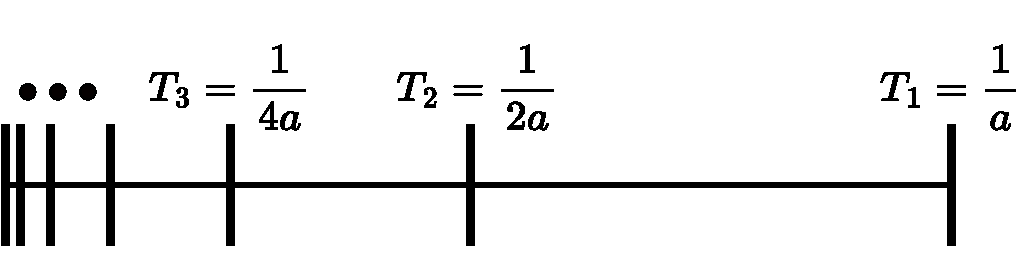
\includegraphics[width=0.8\textwidth]{figures/temperatures.pdf}
    \caption[Temperatures on the lattice]{}
    \label{fig:temperatures_lattice}
\end{figure}
The use of coloured noise allows one to access a wider and finer range of temperatures. In fact, as already mentioned in section \ref{sec:lattice_continuum_}, the temperature on the lattice is given by 
\begin{equation}
    T = \frac{1}{a \, N_t}.
    \label{eq:temperature_lattice}
\end{equation}
Hence one can change temperature either by changing the spacing $a$, or by changing the number points in the time direction $N_t$. 
Both approaches pose serious constraints on the range of accessible temperatures. The spacing $a$ is often determined by the energy scale at which one wants to simulate theory. 
For example in an effective theory, as explained in section \ref{sec:lattice_continuum_}, one has to keep $\Lambda \leq \Lambda_\text{phys}$, and since $a = \pi/\Lambda$, one ends with a constraint on the spacing $a \geq \pi/\Lambda_\text{phys}$. \\
The highest temperature reachable is then limited by mathematical arguments as one cannot have $N_t < 1$, even though in a simulation one often needs $N_t \geq 2$. On the other side the minimum temperature reachable is limited by computational resources as one cannot afford $N_t \to \infty$.
Moreoveor, the resolution of high temperatures is very coarse due to the relation \eqref{eq:temperature_lattice}, in the sense that for small $N_t$, a change in the number of time points causes a significant variation in the temperature. \\~\\
By means of coloured noise one can change the temperature by changing the effective spacing. In fact, if one follows the cooling procedure by keeping $N_t$ fixed, one sets a new temperature which is given by 
\begin{equation*}
    T_\text{eff} = \frac{1}{a_\text{eff} \, N_t} = \frac{1}{sa \, N_t} = \frac{1}{s} \, T,
\end{equation*}
where $s = \Lambda_\text{eff} / \Lambda \leq 1$. Note that not only the temperature has been raised, but one has also gained resolution around $T_\text{eff}$. In fact, to reach this temperature by changing $N_t$, one should change the number of time points to $N_t \to s N_t$, and for what explained before a lower $N_t$ comes with a loss of resolution. \\
The control over temperature will not be investigted in this work. For a more detailed explanation of the procedure and its relevance in the context of the quark-meson model, we refer to \cite{attanasio2022low}.
\newpage
\section{Definition of relevant observables}
\label{sec:observables}
From now on, we will indicate both the dimensionless quantities and dimensionful ones by using the notation of the latters. When beeing on discretised theory, we will be implicitly referring to the dimensionless quantities. A distinction will still be made when relevant. \\~\\
We define the magnetisation $M$ of the field $\phi$ as,
\begin{equation*}
    M = \expect{\frac{1}{V}\sum_n \phi_n}.
\end{equation*}
Thus, in a finite volume lattice system, the absolute magnetisation
\begin{equation*}
    M = \expect{\frac{1}{V}\left|\sum_n \phi_n\right|}.
\end{equation*}
is better suited as an order parameter \cite{friedli_velenik_2017,gattringer_LQCD}. \\
In the continumm, phase transition is characterised by a divergence in the susceptibility, or connected two-points function
\begin{equation*}
    \chi_2 = V \left(\expect{M^2} - \expect{M}^2\right) = V \expect{\left(M-\expect{M}\right)^2}.
\end{equation*}
On a finite volume lattice, one obseres a peak that becomes sharper as the volume is increased. In pratice, the susceptibility of the order parameter 
\begin{equation*}
    \chi_2 = V \expect{\left(M-\expect{|M|}\right)^2}
\end{equation*}
will be adopted. \\
The susceptibility measures the Gaussian fluctuations of the order parameter, the magnetisation. We then introduce the Binder cumulant \cite{binder2010monte}, which quantifies the curtosis of the fluctuations
\begin{equation*}
    U_L \equiv 1 - \frac{1}{3} \, \frac{\expect{M^4}}{\expect{M^2}^2}.
\end{equation*}
It is particular useful to characterise phase transitions in terms of the order parameter $\phi$, since it assummes the values 
\begin{equation*}
    U_L = \begin{cases}0 \quad \hphantom{/3} \text{symmetric phase}, \\ 2/3 \quad \text{broken phase}. \end{cases}
\end{equation*}
We define the fermionic two-points function
\begin{equation} 
\begin{aligned}
    \left\langle \psi(x) \, \bar\psi(y) \right\rangle 
    &= \frac{1}{Z} \, \int \mathcal{D}\phi \, \mathcal{D}\psi \, \mathcal{D}\bar\psi \ \psi(x) \, \bar\psi(y) \, \exp \left( - S_\phi - \psi D \psi + \bar\eta \psi + \bar \psi \eta \right) \\
    &= \frac{1}{Z} \, \int \mathcal{D}\phi \, \mathcal{D}\psi \, \mathcal{D}\bar\psi \ \frac{\delta}{\delta \bar \eta(x)} \frac{\delta}{\delta \eta(y)} \, \exp \left( - S_\phi - \psi D \psi + \bar\eta \psi + \bar \psi \eta \right) \\
    &= \frac{1}{Z} \, \int \mathcal{D}\phi \ \text{det}\left[D(\phi)\right] \ \exp \left( - S_\phi \right) \ \frac{\delta}{\delta \bar \eta(x)} \frac{\delta}{\delta \eta(y)} \, \exp\left( \bar\eta D^{-1} \eta \right) \\
    &= \left\langle \left[D^{-1}(\phi)\right]_{mn}\right\rangle,
\end{aligned}
\label{eq:D_inv_condensate}
\end{equation}
and its connected counterpart
\begin{equation*}
    \left\langle \psi(x) \, \bar\psi(y) \right\rangle_c = \left\langle \psi(x) \, \bar\psi(y) \right\rangle  - \left\langle \psi(x) \right\rangle \, \left\langle\bar\psi(y) \right\rangle .
\end{equation*}
The chiral condensate can then be computed as
\begin{equation*}
    \left\langle  \bar\psi \psi \right\rangle = \underset{n,s}\sum  \left\langle \bar\psi_{n,s} \, \psi_{n,s} \right\rangle = -\underset{n,s}{\tr} \, (D^{-1})_{nn}.
\end{equation*}
On a finite volume lattice, the correlation of a field at two spacetime points is quantified by the correlator
\begin{equation}
    C_\psi(t,0) \equiv \frac{1}{V} \sum_{x} \left[\left\langle \psi(t, \vec{x}) \, \bar\psi(0,0)\right\rangle_c - \left\langle \psi(N_t-t, \vec{x}) \, \bar\psi(0,0)\right\rangle_c \right] .
    \label{eq:correlator_definition}
\end{equation}
Note that we sum up two waves because of the boundary conditions. \\
In momentum space, by using a spectral decomposition, one has
\begin{equation*}
    \begin{aligned}
        \frac{1}{V} \sum_{\vec{x}} e^{-i \vec{p} \vec{x}}\langle\bar\psi(t, \vec{x}) \psi(0, \vec{0})\rangle_c & =\frac{1}{V} \sum_{\vec{x}} e^{-i \vec{p} \vec{x}} \sum_k\langle 0|\bar\psi(t, \vec{x})| k\rangle\langle k|\psi(0, \vec{0})| 0\rangle \\
        & =\frac{1}{V} \sum_{\vec{x}} e^{i \vec{p} \vec{x}} \sum_k\left\langle 0\left|e^{-i p^{\prime} x} \bar\psi(0, \vec{0}) e^{i p^{\prime} x}\right| k\right\rangle\langle k|\psi(0, \vec{0})| 0\rangle \\
        & =\frac{1}{V} \sum_{\vec{x}} e^{-i \vec{p} \vec{x}} \sum_k e^{i k x}\langle 0|\bar\psi(0, \vec{0})| k\rangle\langle k|\psi(0, \vec{0})| 0\rangle \\
        & =\frac{1}{V} \sum_{\vec{x}, k} e^{-i(\vec{p}-\vec{k}) \vec{x}} e^{-E_k t}|\langle 0|\psi(0, \vec{0})| k\rangle|^2 \\
        & =\frac{1}{V} \sum_k \delta(\vec{p}-\vec{k}) e^{-i(\vec{p}-\vec{k}) \vec{x}} e^{-E_k t}|\langle 0|\psi(0, \vec{0})| k\rangle|^2 \\
        & =\frac{1}{V} \sum_n e^{-E_n(\vec{p}) t}\left|\left\langle 0|\psi(0, \vec{0})| p_n\right\rangle\right|^2.
        \end{aligned}
\end{equation*}
Using this, equation \ref{eq:correlator_definition} can be rewritten as
\begin{equation*} 
    \begin{aligned}
        C(t, \vec{p}) & =\frac{1}{V} \sum_{\vec{x}} e^{-i \vec{p} \vec{x}}\left(\langle\psi(t, \vec{x}) \bar{\psi}(0, \vec{0})\rangle_c-\left\langle\psi\left(N_t-t, \vec{x}\right) \bar{\psi}(0, \vec{0})\right\rangle_c\right) \\
        & \propto \sum_n e^{-E_n(\vec{p}) t}-e^{-E_n(\vec{p})\left(N_t-t\right)}=\sum_n 2 e^{-E_n(\vec{p}) \frac{N_t}{2}} \sinh \left[E_n(\vec{p})\left(\frac{N_t}{2}-t\right)\right] .
    \end{aligned}
\end{equation*}
By projecting onto $p=0$, one can note that for large times all the contributions but the ground state are suppressed, so that 
the fermionic correlator assumes the form 
\begin{equation}
    C_\psi(t,0) \approx \sinh \left(E_0^{\psi} \left(\frac{N_t}{2} - t\right)\right),
    \label{eq:correlator_func}
\end{equation}
where $E_0^{\psi}$ is the fermionic mass gap, which will be denoted as $m_{q,\text{phys}}$. \\
An important quantity to compute the correlator on the lattice are the so called time slices
\begin{equation*} 
    S(t, \vec{p})=\frac{1}{V} \sum_{\vec{x}} e^{i \vec{p} \vec{x}} \psi(t, \vec{x}), \qquad \bar{S}(t, \vec{p})=\frac{1}{V} \sum_{\vec{x}} \bar\psi(t, \vec{x}) \, e^{-i \vec{p} \vec{x}}
\end{equation*}
In fact, they are related to the correlator via
\begin{equation*}
    \begin{aligned}
        \left\langle \bar{S}\left(t_1, \vec{p}\right) S\left(t_2,-\vec{p}\right)\right\rangle_c & =\frac{1}{V^2} \sum_{\vec{x}} e^{-i \vec{p} \vec{x}} \sum_{\vec{y}} e^{i \vec{p} \vec{y}}\left\langle\bar\psi\left(t_1, \vec{x}\right) \psi\left(t_2, \vec{y}\right)\right\rangle_c \\
        & =\frac{1}{V^2} \sum_{\vec{x}, \vec{y}} e^{-i \vec{p}(\vec{x}-\vec{y})}\left\langle\bar\psi\left(t_1, \vec{x}\right) \psi\left(t_2, \vec{y}\right)\right\rangle_c \\
        & =\frac{1}{V} \sum_{\vec{r}} e^{-i \vec{p} \vec{r}}\left\langle\bar\psi\left(t_1, \vec{r}\right) \psi\left(t_2, \vec{0}\right)\right\rangle_c \\
        & =C\left(t_1-t_2, \vec{p}\right) .
        \end{aligned}
\end{equation*}
Note that from the second row to the third row translation invariance has been assumed. \\
Using this result, together with \eqref{eq:D_inv_condensate} and \eqref{eq:correlator_func}, one gets to the chain of equalities
\begin{equation*}
    \begin{aligned}
        C_\psi(t, 0) &\approx \sinh\left(m_{q, \text{phys}}\left(\frac{N_t}{2} - t\right)\right) \\
        &= \expect{\bar{S}(t,0) \, S(0,0)} = \frac{1}{V} \,  \sum_n e^{-i \vec p \vec r} \expect{\bar\psi_n \psi_0} = (D^{-1})_{n,0}
    \end{aligned}
\end{equation*}
This allows to compute the correlator on the lattice and extract the physical quark mass via a fiting procedure. Note that we do not need the full inversion of the Dirac operator. One can in fact write 
\begin{equation*}
    (D^{-1})_{n,0} = D^{-1}_{nm} \, \eta_{m},
\end{equation*}
where 
\begin{equation*} 
    \eta_{m} = s \, \delta_{m,0}.
\end{equation*}
is a spinor field where only the component at the origin is non-zero, and are given by the spinor $s$. Hence one is reduced to solve the linear system of equations
\begin{equation*}
    \sum_n D^{-1}_{mn} \, \psi_m = \eta_n,
\end{equation*}
which can be done by means of the Conjugate Gradient algorithm, as detailed in appendix \ref{chap:AppendixC}.\\~\\
By similar arguments one can introduce the bosonic two point function and connected two points function 
\begin{equation*}
    \begin{aligned}
        \expect{\phi(x)\phi(y)} = \frac{1}{Z} \, \int \mathcal{D}\phi \, \mathcal{D}\psi \, \mathcal{D}\bar\psi \ \phi(x) \phi(y) \ e^{-S[\phi, \psi, \bar\psi]} \\
        \expect{\phi(x)\phi(y)}_c = \expect{\phi(x)\phi(y)} - \expect{\phi(x)}\expect{\phi(y)}
    \end{aligned}
\end{equation*}
and arrives at the bosonic correlator 
\begin{equation}
    C_\phi(t,0) \approx \cosh \left(E_0^{\phi} \left(\frac{N_t}{2} - t\right)\right).
    \label{eq:correlator_func_bosons}
\end{equation}
The hyperbolic cosine appears in place of the hyperbolic sine since one applies periodic boundary condition instead of anti-periodic in equation \eqref{eq:correlator_definition}. \\
The last quantity needed in the investigation is the renormalised boson mass, which si defined as 